\documentclass[a4paper,12pt,fleqn]{article}
\usepackage{fixltx2e}
\usepackage[utf8]{inputenc}
\usepackage{graphicx}
\usepackage{sidecap}
\usepackage{fancyhdr}
\usepackage{amssymb,amsmath}
\usepackage[swedish]{babel}
\usepackage[margin=1.5in]{geometry}
\usepackage{abstract}
\usepackage[parfill]{parskip}
\usepackage{tocloft}
\usepackage{adjustbox}
\usepackage{textcomp}
\usepackage[T1]{fontenc}
\usepackage{listings}
\usepackage{xcolor,colortbl}
\usepackage{hyperref}
%----------------------------------------------------------------
%C-kod formatering

\definecolor{listinggray}{gray}{0.9}
\definecolor{lbcolor}{rgb}{0.9,0.9,0.9}
\lstset{
backgroundcolor=\color{lbcolor},
    tabsize=4,    
%   rulecolor=,
    language=[GNU]C++,
        basicstyle=\scriptsize,
        upquote=true,
        aboveskip={1.5\baselineskip},
        columns=fixed,
        showstringspaces=false,
        extendedchars=false,
        breaklines=true,
        prebreak = \raisebox{0ex}[0ex][0ex]{\ensuremath{\hookleftarrow}},
        frame=single,
        numbers=left,
        showtabs=false,
        showspaces=false,
        showstringspaces=false,
        identifierstyle=\ttfamily,
        keywordstyle=\color[rgb]{0,0,1},
        commentstyle=\color[rgb]{0.026,0.112,0.095},
        stringstyle=\color[rgb]{0.627,0.126,0.941},
        numberstyle=\color[rgb]{0.205, 0.142, 0.73},
%        \lstdefinestyle{C++}{language=C++,style=numbers}’.
}
\lstset{
    backgroundcolor=\color{lbcolor},
    tabsize=4,
  language=C++,
  captionpos=b,
  tabsize=3,
  frame=lines,
  numbers=left,
  numberstyle=\tiny,
  numbersep=5pt,
  breaklines=true,
  showstringspaces=false,
  basicstyle=\footnotesize,
%  identifierstyle=\color{magenta},
  keywordstyle=\color[rgb]{0,0,1},
  commentstyle=\color{Darkgreen},
  stringstyle=\color{red}
  }
  %-----------------------------------------------------------------
  %marginaler

  \renewcommand{\abstractnamefont}{\normalfont\normalsize\bfseries}
  \renewcommand{\abstracttextfont}{\normalfont\small}
  \renewcommand{\headrulewidth}{0pt}
  \renewcommand{\cftsecleader}{\cftdotfill{\cftdotsep}} 
  \setlength{\absleftindent}{0pt}
  \setlength{\absrightindent}{0pt}
  \setlength{\headheight}{15pt}

  \addtolength{\oddsidemargin}{-.5in}
  	\addtolength{\evensidemargin}{-.5in}
  	\addtolength{\textwidth}{1in}


  %-----------------------------------------------------------------
  %header and footer

  \pagestyle{fancy}
  \lhead{
  	\begin{picture}(0,0)
  		\put(5,0){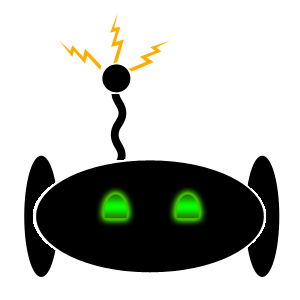
\includegraphics{logotyp.png}}
  	\end{picture}}
	
  \fancyhead[C]{\small{Mapmaster2001}}
  \fancyhead[R]{\small \today}
  \fancyfoot[L]{\small{TSEA56 \\ LIPS Kappa}}
  \fancyfoot[C]{\small{\thepage}}
  \fancyfoot[R]{\small{Projektgrupp 8 \\ mapmaster2001@cyd.liu.se}}

  %-----------------------------------------------------------------

\begin{document}
%-------------------------------------------------------------------
%Första sidan

	\pagestyle{fancy}
\pagenumbering{roman}
	\vspace*{\fill}
		\begingroup
			\begin{center}
				\huge{\textbf{MapMaster 2001}}
				\\
				\vspace{5pt}
				\normalsize
				Kandidatprojekt Y - Grupp 8 - VT2014
				\\
				Version 1.0
				\end{center}
		\endgroup
	\vspace*{\fill}
	
	\begin{center} %Börjar centrering 
		Status
		\\
		\vspace{3pt} %Whitespace 3 pts
	    \begin{tabular}{| p{3cm} | p{3cm} | p{3cm} |} %tabell, 4 horizontella |, 3 cm emellan dem.
	    \hline %översta horizontella linjen.
	    Granskad & - & \today \\ \hline % & -tecken för att "gå till nästa ruta" 
		Godkänd & - & - \\ \hline % avslutas med \\ och \hline.

	    \end{tabular}
	\end{center}
	\vspace{2cm}
	\newpage
%-----------------------------------------------------------------
%Projektidentitet
	
	\vspace*{\fill}
		\begingroup
			\begin{center}
				\LARGE{\textbf{PROJEKTIDENTITET}}
				\\
				\footnotesize
				Grupp 8, 2014/VT, MapMaster2001
				\\
				Linköpings tekniska högskola, ISY
				\\
				\vspace{1cm}
	  \begin{tabular}{| p{3cm} | p{4.3cm} | p{2.4cm} | p{3.8cm} |}
	    \hline
		\textbf{Namn} & \textbf{Ansvar} & \textbf{Telefon} & \textbf{E-post} \\ \hline
	    Jens Edhammer & Dokumentanvsvarig (DOK) & 076-030 67 80 & jened502@student.liu.se \\ \hline
		Erik Ekelund & Designansvarig (DES) & 073-682 43 06 & eriek984@student.liu.se \\ \hline
		David Habrman &  & 976-017 71 15 & davha227@student.liu.se \\ \hline 
		Tobias Grundström & Testansvarig (TES) & 073-830 44 45 & tobgr602@student.liu.se \\ \hline 
		Hans-Filip Elo &   & 073-385 22 32 & hanel742@student.liu.se \\ \hline 
		Niklas Ericson & Projektledare (PL) & 073-052 27 05 & niker917@student.liu.se \\ \hline
	    \end{tabular}
		
		\vspace{1cm}
		\textbf{E-postlista för hela gruppen:} mapmaster2001@cyd.liu.se
		\\[0.5cm]
		
		\textbf{Kund}: Mattias Krysander, Linköpings Universitet, 581 83  LINKÖPING, \\
		013-28 21 98, matkr@isy.liu.se \\
		\textbf{Kontaktperson hos kund}: Mattias Krysander, 013-28 21 98,matkr@isy.liu.se 
		\\
		\textbf{Kursansvarig}: Tomas Svensson, 3B:528,013 28 21 59,tomass@isy.liu.se
		\\[0.5cm]
		\textbf{Handledare}: Peter Johansson, 013-28 1345 peter.a.johansson@liu.se

				\end{center}
		\endgroup
	\vspace*{\fill}
\newpage

%-----------------------------------------------------------------
%Innehållsföreteckning

\addto\captionsswedish{\renewcommand{\contentsname}{Innehållsförteckning}}

\tableofcontents
\thispagestyle{fancy}
\newpage

\pagenumbering{arabic}
%-----------------------------------------------------------------
%Översikt

\section{Inledning}
%''Ge en översiktlig beskrivning av produkten och uppdraget gärna kopplat till bilder.
%Lyft gärna fram det som ni anser är utmanande/intressant i uppdraget. 
%Beskriv kortfattat dispositionen på rapporten.''

En robot med tillgång till ett antal avståndssensorer, ett gyro och en RFID-sensor placeras i ett stängt område med dimension 6x6 meter som är uppdelat i 40x40 centimeters segment. 
Den ska, med en vägg som startpunkt, helt autonomt kartlägga området genom att markera ut var väggar finns och var det finns områden som inte går att nå. 
Den ska även markera ut var det går att finna RFID-taggar, som symboliserar brandhärdar. 
Om inte hela det slutna området är kartlagt ska den upptäcka vilka segment som är oupptäckta, färdas dit och lägga till det i kartan. 
När hela området är kartlagt ska roboten ta sig tillbaka till startpunkten och avsluta arbetet. Ett exempel på en karta kan ses i Figur \ref{fig:omrade}.
\begin{figure}[htp] %Placera här om det finns plats, annars så snart som möjligt, på toppen av en sida.
  \begin{center}
  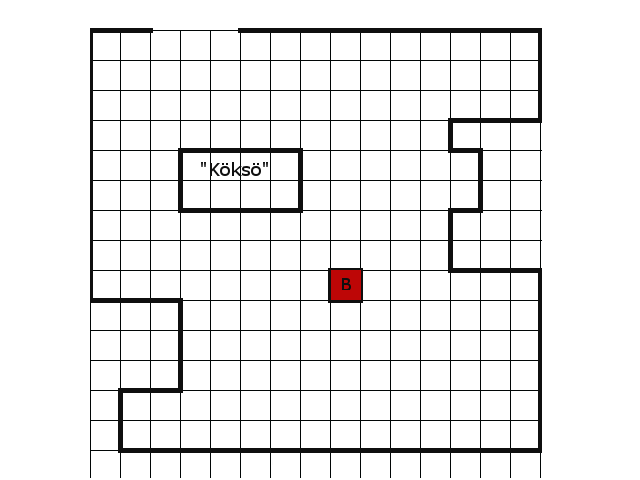
\includegraphics[keepaspectratio=true,scale=0.5]{gimpmap.png}  %skala och filnamn. 
  \end{center}
  \caption{Exempel på område som ska kartläggas} %figurtext.
  \label{fig:omrade}
\end{figure}

Stora delar av arbetet med denna produkt består av att utnyttja den teoretiska kunskap som finns och att koppla den till praktiken för att sedan implementera principerna på roboten. 
Detta innefattar bland annat reglerteori, sannolikhetslära och matematisk analys.

En av de största utmaningarna med robotens uppdrag är dock att rita ut en karta över området utan att veta var den befinner sig - men hur går det att veta var roboten befinner sig utan en karta? 

\section{Problemformulering}
%Redogör kort för kravbilden och referera till projektdirektiv och kravspecifikation för %att läsa detaljer.
%Lägg återigen mest fokus på det som ni ansåg utmanande/intressant.

Den slutgiltiga produkten ska uppfylla ett antal krav (Se Kravspecifikation) för att godkännas av beställaren. 
Kraven som ställts är delvis baserade på vad beställaren ville få levererat (Se Projektdirektiv för kartrobot) och delvis på sådant som projektgruppen ansåg var viktigt för robotens funktionalitet. 
Sammanfattningsvis består kraven bland annat av de delar som beskrivs av scenariot i inledningen. Den innehåller även en del krav på vilka delprodukter som ska vara klara vid vissa specifika datum.

\section{Kunskapsbas}

%%Här behövs lite referenser sen
Den litteratur som använts under projektets gång består till stor del av böcker inom grunderna för bland annat sannolikhetslära, datorteknik, elektronik, reglerteknik och matematisk analys. 
Dessa har kombinerats med datablad för de komponenter som använts tagna från ISY:s sida VanHeden\footnote{\url{https://docs.isy.liu.se/twiki/bin/view/VanHeden}} och datablad från Atmel för 
de processorer som modulerna baserats på\footnote{\url{http://www.atmel.com/images/doc8059.pdf}}. 
Utöver detta har även diverse forum på internet berörande exempelvis \emph{C}-,\emph{C++}-\footnote{\url{http://stackoverflow.com/}} och \emph{AVR}-programmering\footnote{\url{http://www.avrfreaks.net/}} besökts.

\section{Genomförande}
%Beskriv hur projektet har bedrivits och referera bland annat till LIPS-modellen, %systemskiss, projektplan och designspecifikation. Observera att designspecifikationen %belyser arbetsprocessen och inte den slutliga produkten så om ni uppdaterat %designspecifikationen löpande under projektet så kan ni infoga t ex den version som var %aktuell vid BP3.

Det grundläggande upplägget på projektet har baserats på LiPS-modellen, det vill säga de olika faserna i arbetet och vad som bör göras. 
De dokument som producerades under för-fasen så som systemskiss och projektplan skrevs gemensamt för att alla medlemmar skulle få en så bra inblick som möjligt i hur arbetet planerades. 
För mer detaljerad beskrivning av arbetsupplägget hänvisas läsaren till ovan nämnda dokument (Se Systemskiss och Projektplan).

Projektet har delats upp i mindre delprojekt som olika projektmedlemmar fått ansvara för. 
Det har bland annat inneburit förberedande design av delprodukt (Se Designspecifikation) och implementering. 
Vid ett delprojekts slutförande har hårdvaran eller den skrivna koden förklarats för de andra projektmedlemmarna och sedan slagits samman med resten av projektet. 

För att på ett smidigt vis slå samman kod och möjliggöra simultan programmering har en versionshanteringstjänst vid namn Github använts. 
När hårdvara skulle utvecklas delades projektgruppen in modulvis, två personer per modul.
Dialog hölls mellan grupperna för att säkerställa att portar och kontakter placerades på smidiga ställen.

Längre in i projektet ändrades grupperna något för att ge alla projektmedlemmar en chans att arbeta med varandra, men även för att det var färre delmoment att arbeta med. 
I slutfasen av projektet turades gruppmedlemarna om att skriva den tekniska dokumentationen medan andra arbetade med roboten för att effektivisera arbetet.

\section{Teknisk beskrivning}
%Redovisa det tekniska resultatet och skrivuppgifterna på ett lämpligt sätt. Detaljerade beskrivningar på grindnivå i hårdvaran eller på instruktionsnivå i mjukvaran är i detta sammanhang oftast ointressant. Referera den tekniska dokumentationen och skrivuppgifterna för beskrivning av detaljer. Lyft fram egna kreativa lösningar!



\subsection{Kommunikation mellan processorer}
Kommunikationen mellan processorerna sker via en Serial Peripheral Interface Bus, hädanefter refererad till som en SPI-buss.
Roboten är konstruerad med tre processorer på två separata vir-kort och kopplas ihop med hjälp av en bandkabel. På roboten agerar kommunikationsmodulen master och de övriga två modulerna är slaves. SPI-bussen kan sammanfattas till att master skiftar ett 8 bitars register med en slave. SPI-bussen har alltså möjlighet för duplex dataöverföring. För ytterligare detaljer angående SPI-bussen se den tekniska dokumentationen.

När master väljer en slave, genom Slave Select signalen, genereras ett avbrott på slave-processorn. Detta innebär att master kan skicka hämta data i princip var som helst i ett program på en slave-processor. För kommunikations som måste initieras från slave till master har vi kopplat en avbrottssignal som säger till master-processorn att påbörja SPI-kommunikation med aktuell slave-processor.

\subsubsection{Datahantering}
För att avbrotten ska bli så korta som möjligt på processorn så har datahanteringen på kommunikationsmodulen flyttats ut ur avbrott. Anledningen till detta är att så länge processorn befinner sig i avbrott skulle vidare avbrott kunna missas. Sanningsvariabler ifall ny data finns tillgänglig för datahantering används istället. Dessa sanningsvariabler avläses i master-processorns main-loop, vilket visas i flödesdiagrammet i figur~\ref{fig:SPIrec}. Detta ger att nya mottagningar kan påbörjas medan data behandlas, man får dock beakta att data i en given buffer måste behandlas innan den skrivs över av nästa kommunikation.

\begin{figure}[htp] %Placera här om det finns plats, annars så snart som möjligt, på toppen av en sida.
  \begin{center}
  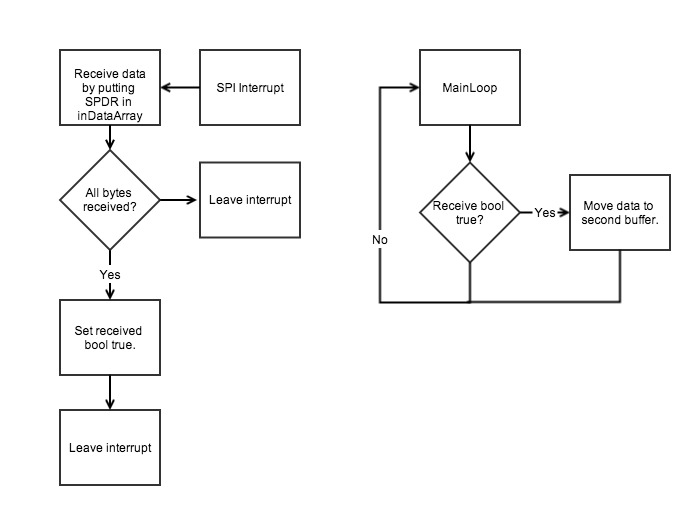
\includegraphics[keepaspectratio=true,scale=0.5]{spirec.jpg}  %skala och filnamn. 
  \end{center}
  \caption{Flödesdiagram för bussmottagning} %figurtext.
  \label{fig:SPIrec}
\end{figure}


\subsubsection{Databufferstruktur}
För att undvika ovannämnda problem utnyttjas en dubbelbuffer. Första buffern är mottagningsbuffern inuti buss-avbrottet. När vi når en databehandlingsfunktion flyttas denna data över till en ny buffer under datahanteringen. Detta innebär att vi kan ta emot ny data från samma sändare på samma buffer sålänge vi har påbörjat databehandling.

\subsection{Kommunikation melllan PC och robot}
\subsection{PC-mjukvara med grafiskt gränssnitt}
\subsection{Pulse Width Modulation}

För att styra chassits motorer används AVR-processorn inbyggda pulsbreddsmodulering, PWM. 

\subsection{LCD-display}
\subsection{Kartabstraktion}

En karta abstraheras i form av en rektangel med ett rutnät med dimensionen 33x17 rutor med koordinaterna (0,0) i det övre vänstra hörnet. Det verkliga området skulle med liknande rutnät bli 15x15 rutor. För att kompensera för eventuella mätfel utökas matrisen något för att underlätta uppritningen. Felaktigheter i avläsning kan leda till att roboten i abstraktionen tillfälligt är utanför sitt givna område. Roboten kommer i början att placeras i punkten (16,0) och rita upp kartan utifrån detta. Det kommer då inte spela någon roll hur roboten är placerad i det verkliga systemet eftersom det finns utrymme för 15 rutor åt båda hållen inklusive marginaler. 

En abstraktion av en matris i mjukvara skapas med hjälp utav nästlade arrayer, eller någon modern motsvarighet. I utvecklingsmiljön Atmel Studio finns språket C++ tillgängligt, men däremot ej C++ standardbibliotek med abstraktioner.

\subsubsection{Objektklasser}

Kartmatrisen hålls inne i en containerklass med funktioner för att abstrahera access till den. I modern programmering är objekthantering ett kraftfullt verktyg för abstraktion. Klasserna som används följer nedan, med engelska namnet inom parantes.

\begin{itemize}
	\item Karta (Map)
	\item Kartsektion (MapSection)
	\item Robot (Robot)
\end{itemize}

I C++-implementeringen är Robot en dotterklass till MapSection. Detta då alla objekt i en matris måste vara av samma objekttyp. Roboten ärver då vissa egenskaper från MapSection - men innehåller klart mer logik för att hantera positionering och kartläggning. 

MapSection kan anta ett antal olika tillstånd för att markera vilken typ av område det är. Nedan följer de tillstånd som implementerats i klassen MapSection: 

\begin{itemize}
	\item Stängt område (Closed)
	\item Outforskat område (Unexplored)
	\item Tomt område (Empty)
	\item Brandhärd (Fire)
\end{itemize}

Till en början är alla områden outforskade. I takt med att sensordata kommer in och beräknas kan sedan roboten omvandla tillstånden hos objekten i kartan utefter given logik. 

\subsection{Sensormodul}
Roboten har nio olika sensorer. En RFID-läsare, ett gyroskop, en reflexsensor, en långdistansmätare, en mellandistansmätare och fyra kortdistansmätare. 
RFID-läsaren ger ut en digital signal och behandlas med USART. Vid detektion av en RFID-tagg så stängs USART-avbrott av och ett kommando skickas till styrmodulen som säger till att vi hittat en brandhärd. 
USART-avbrotten stängs av för att inte låsa sensormodulen med flera läsningar av samma tagg. Avbrottet tillåts då roboten lämnat segmentet genom att styrmodulen skickar ett kommando till sensormodulen.
De resterande sensorerna ger analoga utsignaler och behandlas med hjälp av en intern A/D-mux på sensormodulen. 
Sensormodulen hämtar kontinuerligt signaler från avståndssensorerna, genom att stega igenom muxen, och från alla sensorer genom att stega igenom muxen. Den hoppar, i grundtillståndet, över gyroskopet och reflexsensorn. 
Mätningar på gyroskopet görs på begäran av styrmodulen och låser sensormodulen till enbart gyroskopmätningar. 
Läsningen slutförs när roboten svängt 90 grader och sensormodulen skickar ett kommando till styrmodulen som säger att svängen är klar. 
Även reflexsensorn körs på begäran av styrmodulen men låser inte sensormodulen. Reflexsensorn tas istället med i muxräkningen. 
Detta för att styrmodulen fortfarande behöver kontinuerliga sensorvärden från avståndssensorerna. Läsningar från reflexsensorn upphör då roboten färdats $40$ cm och sensormodulen skickar ett kommando till styrmodulen
som säger att roboten nått ett nytt segment.

\subsubsection{AD-omvandling}

\subsection{SLAM}


\section{Resultat}
Beskriv kortfattat hur produkten används, hänvisa till användarmanualen.
Beskriv vilken prestanda produkten har och hur det har testats, hänvisa till eventuella testprotokoll.
Kommentera om produkten klarade de kraven som ställdes upp i kravspecifikationen. 
\section{Slutsatser}
Slutsatser
Sammanfatta arbetet. 
Lyft fram det ni är mest nöjda med.
Reflektera över resultatet såväl tekniskt som över genomförandet. Referera efterstudien.
Framtida arbete
Vad skulle ni göra annorlunda om ni skulle göra om samma uppdrag?
Vad skulle ni vilja utveckla om ni fick mer tid?
Hur skulle ni tänka er att ändra uppgiften för att göra den ännu mer intressant?
\section{Referenser}


% ----------------------------- Appendix -----------------------------------------
% --------------------------------------------------------------------------------

\newpage
\appendix
\pagestyle{empty}
\newgeometry{left=2cm,right=2cm,bottom=2cm,top=2cm}
\section{Appendix A}
LIPS-dokument och fördjupningar enligt ovan.
\end{document}